\documentclass[11pt,a4paper]{article}

\usepackage[utf8]{inputenc}
\usepackage[T1]{fontenc}

%%%%%%%%%%% Own packages
\usepackage[a4paper, margin=1in]{geometry}
\usepackage{multicol}

% Boxing
\usepackage[most]{tcolorbox}
\tcbset{enhanced}
%\usepackage{capt-of}	% captions in boxes

% Header/footer
\usepackage{fancyhdr}
\pagestyle{fancy}
\renewcommand{\headrulewidth}{0pt}

% Listsings and items
\usepackage[shortlabels]{enumitem}
\setenumerate{wide,labelwidth=!, labelindent=0pt}
\usepackage{varioref}
\usepackage{hyperref}
\usepackage{cleveref}

% Maths
\usepackage{physics}
\usepackage{cancel}
\usepackage{amstext,amsbsy,amssymb}
\usepackage{times} 
\usepackage{siunitx}
\usepackage{tensor}

%% Graphics
\usepackage{caption}
\captionsetup{margin=10pt,font=small,labelfont=bf}
%\renewcommand{\thesubfigure}{(\alph{subfigure})} % Style: 1(a), 1(b)
%\pagestyle{empty}
\usepackage{graphicx} % Include figure files

\title{AST4320\\ 
\vspace{5mm}Assignment 3}
\author{Jakob Borg}
%%%%%%%
\begin{document}
%%%%%%%

\maketitle

%\lhead{Jakob Borg}
\lhead{Assignment 3 AST4320}
\rhead{Jakobbor}
%%%%%%%%

\section*{Exercise 1}
\begin{itemize}
% DOT 1
\item Assuming only hydrogen and helium, with fractions $\mathit{X}=0.76$ and $\mathit{Y}=0.24$ respectively. The mean molecular weight is given by 

\begin{equation}
\mu = \frac{1}{\sum_j \frac{X_j}{A_j}}
\end{equation}
where $X_j$ is the mass fractions for element $j$ and $A_j$ is the fraction of atomic weight in terms of the hydrogen mass over the total number of particles provided to the gas by element $j$. This will change dependent on the ionization fraction of the gas. For either neutral or fully ionized gas this is simple to compute for a primordial gas (only hydrogen and helium)
\begin{align}
A_\mathit{X} &=
    \begin{cases}
        &\frac{1}{1} \qq{neutral}
        \\
        &\frac{1}{2}\qq{ionized}
    \end{cases}
& 
A_\mathit{Y} &=
    \begin{cases}
    & \frac{4}{1}  \qq{neutral}
    \\
    &\frac{4}{3} \qq{ionized}
    \end{cases}
\end{align}
So assuming the IGM is either neutral or fully ionized we get two different mean molecular weights
\begin{align}
\mu_\text{neutral} &= \frac{1}{\mathit{X}+ \frac{\mathit{Y}}{4}} = 1.21951\approx 1.22
\label{eq:mu_neutral}
\\
\mu_\text{ionized} &= \frac{1}{2\mathit{X}+ \frac{3\mathit{Y}}{4}} = 0.58823 \approx 0.59
\label{eq:mu_ion}
\end{align}

% DOT 2
\item
The Jeans lengths given as
\begin{equation}
\lambda_J = c_s \sqrt{\frac{\pi}{G\rho}}
\label{eq:Jeans_length}
\end{equation}
where $c_s$ is the speed of sound given as
\begin{equation}
c_s = \sqrt{\frac{k_B T}{\mu m_p}}
\label{eq:Sound_speed}
\end{equation}
and $\rho$ is the density of the medium. Considering the IGM we are looking at the baryonic matter, so the density will be
\begin{equation}
\rho = \rho_b = \rho_{b,0}(1+z)^3 = \Omega_{b,0}\rho_{c,0}(1+z)^3
\label{eq:rho_b}
\end{equation}
where we have used
\begin{align*}
\Omega_{b,0} &= \frac{\rho_{b,0}}{\rho_{c,0}} = 0.048
\\
\qq*{where} \rho_{c,0} &= \frac{3H_0^2}{8\pi G} \approx \SI{8.64e-30}{g.cm^{-3}}.
\end{align*}
Now we can combine \cref{eq:Sound_speed,eq:rho_b} into \cref{eq:Jeans_length} to find the Jeans length of the IGM as a function of redshift and temperature
\begin{align*}
\lambda_J &= \sqrt{\frac{k_BT\pi}{\mu m_p G \rho}}
\\
&= \sqrt{ \frac{k_B T\pi}{\mu m_p G \Omega_{b,0} \rho_{c,0} }}(1+z)^{-\frac{3}{2}}
\end{align*}
Inserting the following values assuming ionized IGM at redshift 4
\begin{align*}
k_B &= \SI{1.38e-16}{cm^2.g.s^{-2}.K^{-1}} & T &= \SI{1e4}{\kelvin} & z&=4
\\
\mu &= 0.59 & m_p &= \SI{1.67e-24}{\gram} & G&= \SI{6.67}{\cubic\cm\per\gram\per\square\second}
\end{align*}
we find a value for the Jeans length, and corresponding wave number
\begin{align*}
\lambda_J &= \SI{1.1298e24}{\cm} & k &= \frac{2\pi}{\lambda_J} = \SI{5.5615e-24}{\cm^{-1}}
\end{align*}

% DOT 3
\item The velocity width in redshift-space is the difference in velocity of the different sides of a region. Assuming the velocity is only provided by the Hubble flow
\begin{equation}
v = Hr
\label{eq:Hubble_flow}
\end{equation}
we can find the velocity of the different parts of the IGM. Assuming spherical symmetric gas at a distance $r$ with diameter equal the Jeans length, the difference in velocity along the line of sight will be
\begin{align}
\Delta v(z) &= H(z) \left[\left(r+\frac{\lambda_J}{2}\right) - \left(r - \frac{\lambda_J}{2}\right)\right]
\\
&= H(z) \lambda_J
\\
\qq*{where} H(z) &= H_0 \sqrt{\Omega_m(1+z)^3+\Omega_r(1+z)^4+\Omega_\Lambda} \qq{from Friedmann} \label{eq:Friedmann}
\end{align}
Using the same redshift, $z=4$ we find
\begin{align*}
\Delta v(z=4) &= \SI{2.2e-18}{\s^{-1}} \sqrt{4^3\cdot0.308+0.692}\cdot \SI{1.1298e24}{\cm}
\\
&\approx \SI{1.123e7}{\cm\per\s}
\end{align*}

%DOT 4
\item 
The width of the Ly$\alpha$ extinction depends on the size of the IGM, or the more precisely the optical depth. For small optical depths the absorption features will be mostly a Gaussian profile. For increasing optical depth the extinction profiles becomes more saturated, and eventually the Lorentzian wings of the extinction profile will be visible in the absorption features for high optical depth.

% DOT 5
\item The thermal broadening scale of the Ly$\alpha$ extinction profile is given as
\begin{equation*}
v_\text{th} = \sqrt{\frac{2k_B T}{m}}
\end{equation*}
where $m$ supposedly is the <<mass of the particle>>. As we have both helium and hydrogen, we use the mean particle mass $m= \mu m_p$ here. Assuming ionized IGM with the usual temperature $T=\SI{1e4}{K}$ we find a thermal broadening scale
\begin{align*}
v_\text{th} &= \sqrt{\frac{2k_B T}{\mu m_p}}  = \SI{1.674e6}{cm.s^{-1}}.
\end{align*}
This is similar to the velocity width from the Hubble flow. The fraction of the two gives
\begin{align*}
\frac{\Delta v(z=4)}{v_\text{tf}} &= 6.708
\end{align*}
but this fraction changes dependent on the redshift we use in the Hubble flow, and so at a lower redshift the comparison will be even closer before $\Delta v(z)$ becomes smaller than the thermal broadening scale at low redshift.
\end{itemize}

\section*{Exercise 2}
Using the expression from the lecture notes we have the integral
\begin{equation}
\tau_e(z) = c \sigma_T \int_0^z \frac{n_e(z) \dd{z}}{(1+z)H(z)}
\end{equation}
where the speed of light and the Thompson scattering cross section are constants. Assuming the IGM is highly ionized and only consisting of hydrogen, we approximate the electron density with the hydrogen density $n_e \approx \bar{n}_H = \SI{1.9e-7}{\per\cubic\cm}(1+z)^3$. The Hubble parameter is found using \cref{eq:Friedmann} with parameters $\Omega_\Lambda = 0.692,\, \Omega_m = 0.308, \, \Omega_r = 0$.

The integral is solved numerically in the python script \textit{exe2.py}. Here we solve the integral by looping over $z$ values in the range $z\in [0,10]$. The value at some specifically interesting redshifts ($z = [0,6,10]$) is also printed and we plot the hole result in \cref{fig:optical_depth}. We find values
\begin{align*}
\tau_e(z=0) &= 0
\\
\tau_e(z=6) &= 0.0347 \approx 0.04 \qq{as in lecture notes}
\\
\tau_e(z=10) &= 0.0718
\end{align*}

\begin{figure}
\centering
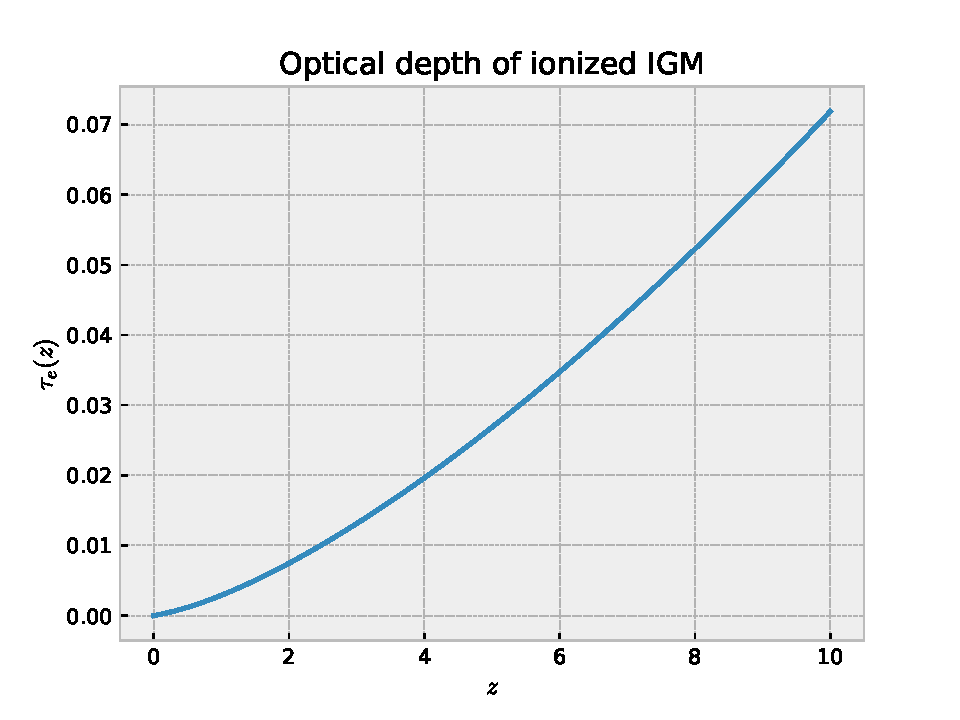
\includegraphics[width=0.8\linewidth]{optical_depth_exe2.pdf}
\caption{Optical depth of fully ionized IGM of only hydrogen as a function of redshift in the range ${z\in[0,10]}$.}
\label{fig:optical_depth}
\end{figure}

\section{Exercise 3}
Second order differential equation from lectures for density assuming isothermal halo
\begin{equation}
-\frac{k_B T}{m_\text{DM}r^2}\dv{r^2}{r}\dv{\ln(\rho)}{r} = 4\pi G \rho.
\label{eq:ODE}
\end{equation}
\begin{itemize}
% DOT 1
\item We show that the given expressions provide solutions to \cref{eq:ODE} by insertion.
\begin{gather*}
\rho = \frac{A}{r^2}  A = \frac{k_B T}{2\pi G m_\text{DM}}
\\
\qq*{rewrite derivatives} \dv{\ln(\rho)}{r} = \frac{1}{\rho}\dv{\rho}{r} = \frac{r^2}{A}\dv{r} \left(\frac{A}{r^2}\right) = - 2 r^{-1}
\end{gather*}

\end{itemize}
\end{document}

























